\newpage
%%%%%%%%%%%%%%%%%%%%%%%%%%%%%%%%%%%%%%%%%%%%%%%%%%%%%%%%%%%%%%%%%%%%%%%%%%%%%%%%
%%%%%%%%%%%%%%%%%%%%%%%%%%%%%%%%%%%%%%%%%%%%%%%%%%%%%%%%%%%%%%%%%%%%%%%%%%%%%%%%

\section{\textcolor{red}{Aspectos da musicalidade na dança}}
\label{sec:aspectosusicalidade}
Ver Figura \ref{fig:aspectos-musica}.
\begin{figure}[h!]
    \centering
    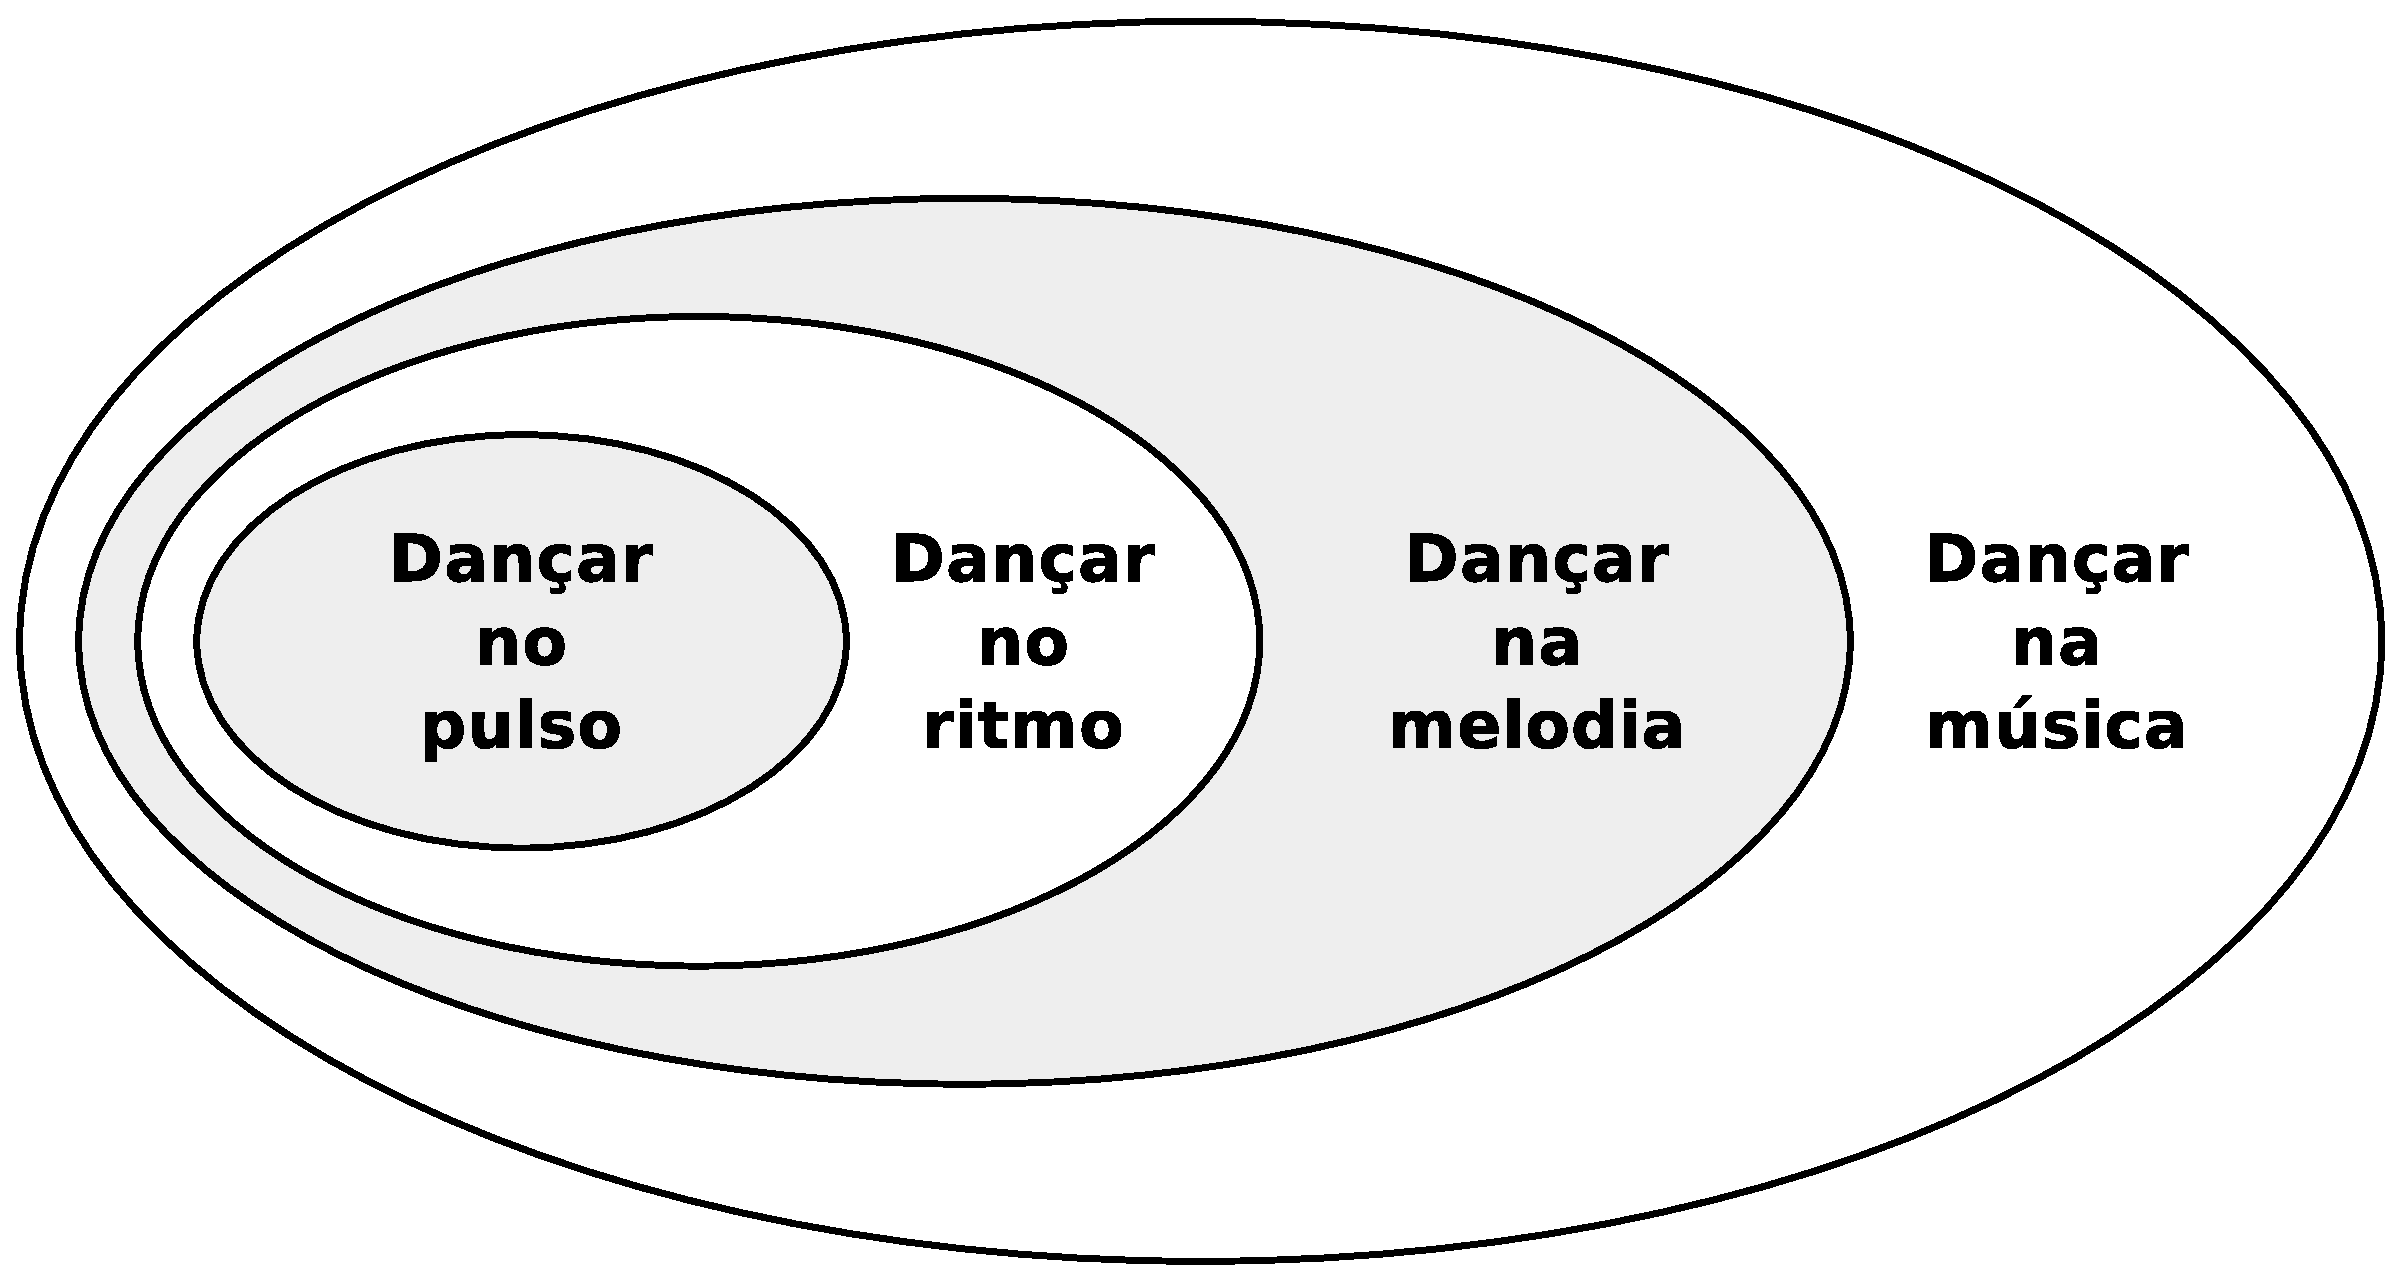
\includegraphics[width=\textwidth]{chapters/cap-musicalidade-tecnica/aspectos-musica.eps}
    \caption{Aspectos da músicalidade na dança.}
    \label{fig:aspectos-musica}
\end{figure}

\subsection{\textcolor{red}{Dançar no pulso}}
Ver Figura \ref{fig:lamentoconsolopulso1}.
\begin{sidewaysfigure}
    \centering
    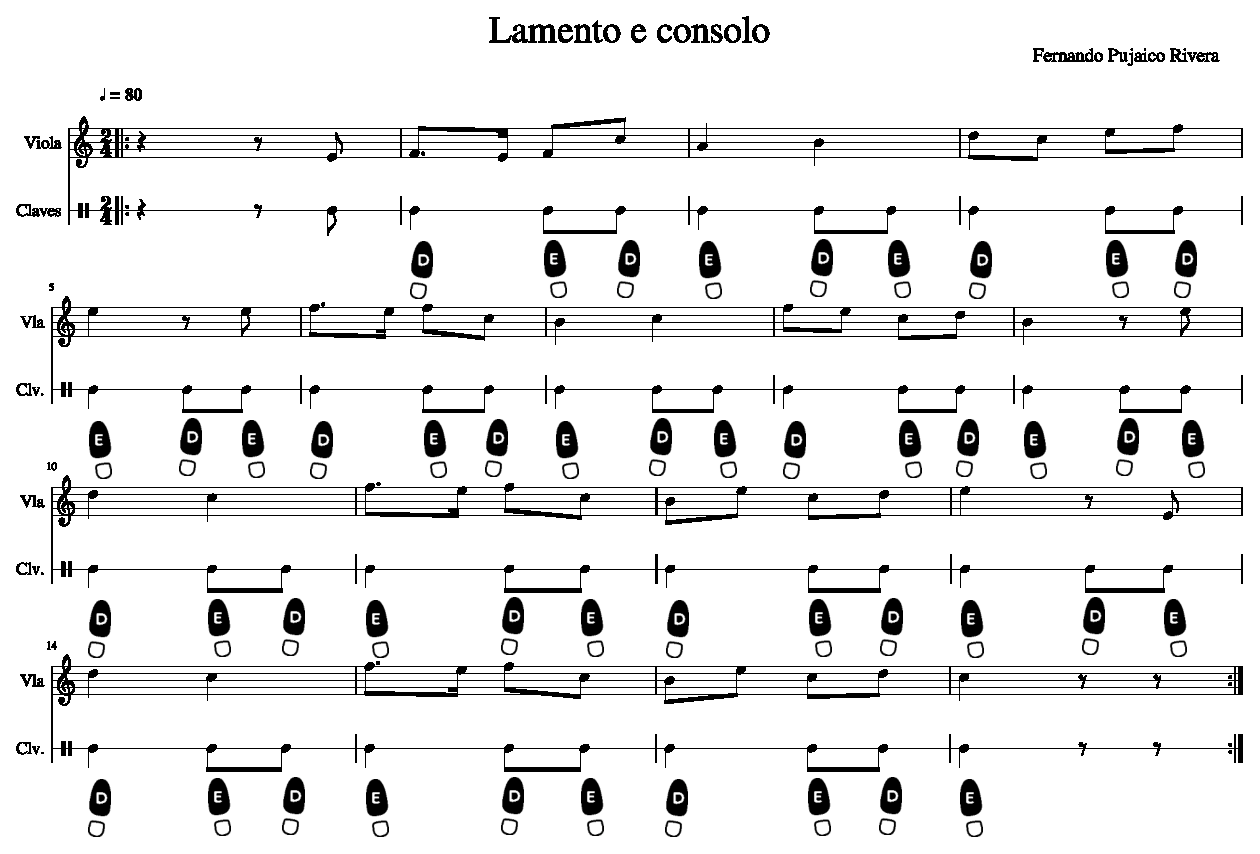
\includegraphics[width=\textwidth]{chapters/cap-musicalidade-tecnica/lamento-e-consolo-clave-pulso-1.eps}
    \caption{Música dançada no pulso.}
    \label{fig:lamentoconsolopulso1}
\end{sidewaysfigure}

Ver Figura \ref{fig:lamentoconsolopulsobreak1}.
\begin{sidewaysfigure}
    \centering
    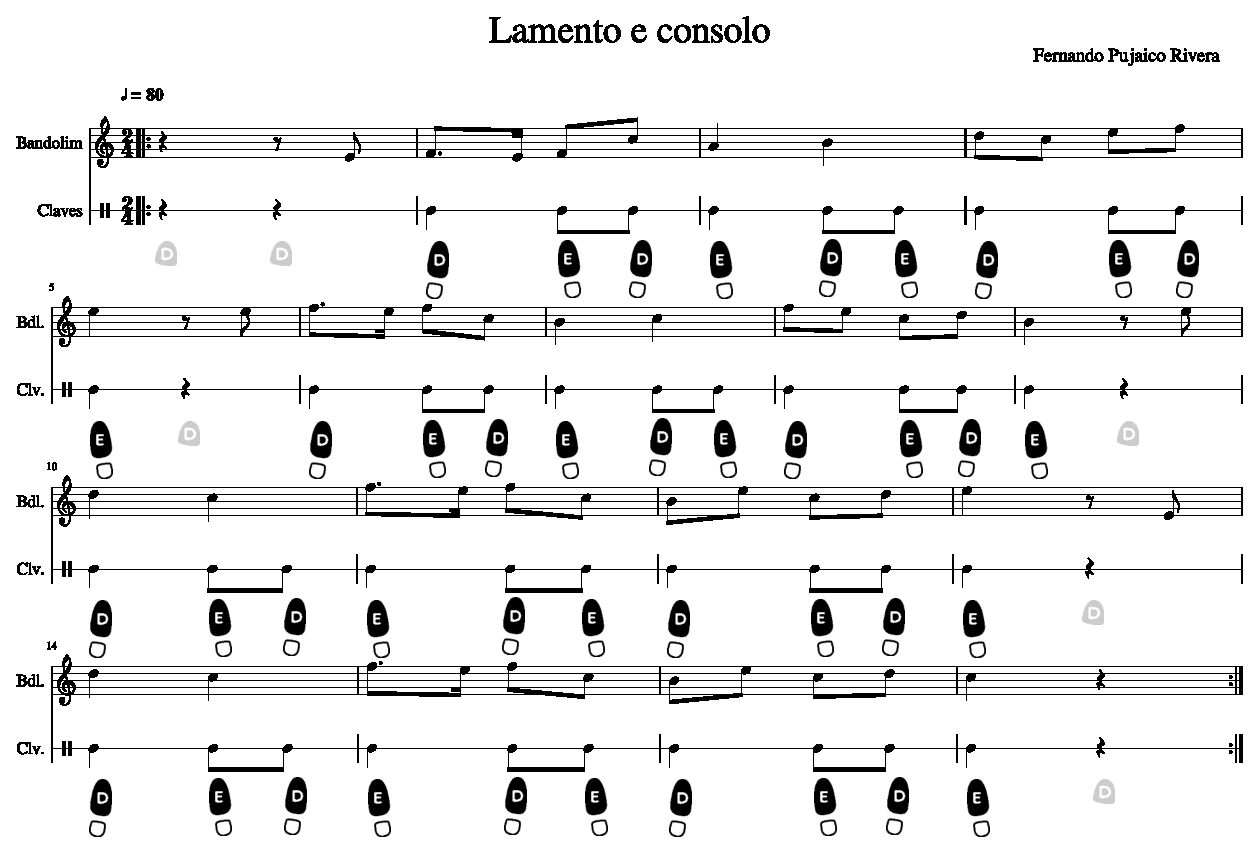
\includegraphics[width=\textwidth]{chapters/cap-musicalidade-tecnica/lamento-e-consolo-clave-pulso+break-1.eps}
    \caption{Música dançada no pulso e usando breaks.}
    \label{fig:lamentoconsolopulsobreak1}
\end{sidewaysfigure}


\subsection{\textcolor{red}{Dançar no ritmo}}
Una buena regla general, especialmente si es nuevo en el baile, es mantener el pulso o el ritmo en su cuerpo.

Mantener el pulso o el ritmo en la cabeza o en el pecho es una de las cosas más fáciles para cualquier persona.

%https://tangowords.wordpress.com/2017/01/10/elements-of-musicality-beat-and-rhythm/
\begin{comment}
quando começamos a dançar, aprendemos a dançar com o batida, 
depois de um tempo começamos a dançar com o ritmo, eventualmente descobrimos como dançar com a música. 
Claro, estes não são separados; Quando dançamos ao ritmo, 
também dançamos ao  batida. 
E quando dançamos a música, os elementos de batida e ritmo também estão lá.

Ao falar com os dançarinos, acho que às vezes há confusão entre batida e ritmo. 
Simplificando, a batida é o pulso constante que você sente na melodia, 
como um tique-taque do relógio. É com o que você pode bater palmas ou bater o pé em. 
O ritmo é o padrão real que as notas de comprimentos diferentes fazem, 
que em uma música podem ser as mesmas que os padrões de palavras. 
Além do tamanho das notas, o ritmo também é criado quando algumas notas são enfatizadas sobre outras.

Geralmente, a dance music (exceto valsa / vals, claro) tem quatro batidas no bar. 
As batidas 1 e 3 são as batidas fortes (o compás no tango) as batidas 2 e 4 
são as batidas fracas (às vezes chamadas de batidas de costas ou de batidas). 
Em seu nível mais simples, quando dançamos, tendemos a pisar nas batidas 1 e 3. 
(Embora, ao bater palmas, a preferência seja aplaudir a batida de trás).

Claro, tudo isso se aplica a qualquer dança criativa de parceiros, 
não apenas ao tango. Em algumas aulas, às vezes você ouve: 
"Este é um movimento de seis batidas" ou "Este é um movimento de doze batidas". 
Isso só é verdade se você estiver se limitando a dançar mecanicamente e unicamente 
ao batida da música. Se você está dançando ao ritmo, 
quantas batidas levará dependendo de como você trabalha com a música.

É muito fácil cair na armadilha de pensar em padrões de passos e se tornar um 
"dançarino de um e três". (E, infelizmente, a batida fortemente acentuada de boa 
parte do que se passa por dance music tende a encorajar isso ... mas isso é outra 
história para outro post no blog!) Somos dançarinos, não metrônomos.
\end{comment}

Ver Figura \ref{fig:lamentoconsoloritmo1}.
\begin{sidewaysfigure}
    \centering
    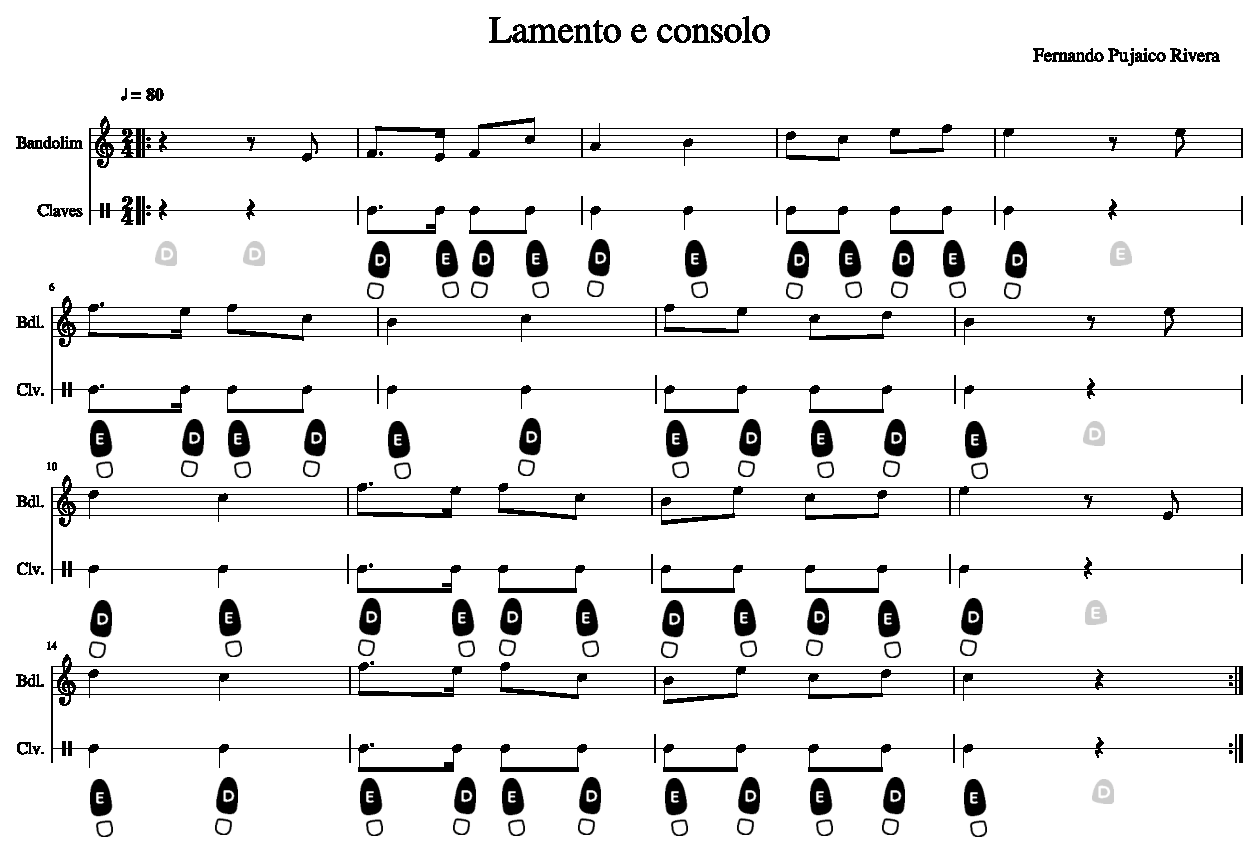
\includegraphics[width=\textwidth]{chapters/cap-musicalidade-tecnica/lamento-e-consolo-clave-ritmo-1.eps}
    \caption{Música dançada no ritmo.}
    \label{fig:lamentoconsoloritmo1}
\end{sidewaysfigure}

\subsection{\textcolor{red}{Dançar na melodia}}
Para darle un poco más de libertad y creatividad, 
mantener el pulso o el ritmo en sus pies le brinda la capacidad de interpretar 
la melodía con el resto de su cuerpo, si así lo desea.

todas as nuances do vocal podem ser seguidos, 
isso vai variar muito de pessoa ou quando se é uma coreografia é escolha do coreografo, 
eu sigo a velocidade do canto e a intensidade da mesma

\subsection{\textcolor{red}{Dançar na música}}

